\documentclass[../main/git_course_main.tex]{subfiles}
\begin{document}

\setcounter{chapter}{3}
\chapter{Branches}

\section{Overview}

In this chapter, you will learn:

\begin{itemize}
	\item What branches are in Git and how they are useful
	\item How to create branches
	\item How to merge branches back into your main branch
	\item How to handle conflicting file changes when merging branches
\end{itemize}

\section{What are branches?}

A \verb$branch$ in Git allows you to work in parallel on different features before integrating them into your main branch (commonly the \verb$master$ branch).

Often, the the \verb$master$ branch is used for stable versions of the program. Branches can be used to develop features independently without disrupting the stable version. The branches are then integrated back into the master when the feature is completed.

\section{Creating a branch}

In this section we will demonstrate the process of creating a new branch and use it to develop a feature which finally is merged back into the \verb$master$. Figure \ref{fig:state_before_branching} shows the state of the repository before creating the branch. 

\begin{figure}[h!]
\begin{redbox}
Our example repository have backed up to the third commit of our repository (the state after Chapter 2) in order to make it easier to visualize. If you are following along, you can simply continue developing on the last commit.
\end{redbox}
\end{figure}

\begin{figure}[h!]
	\centering
	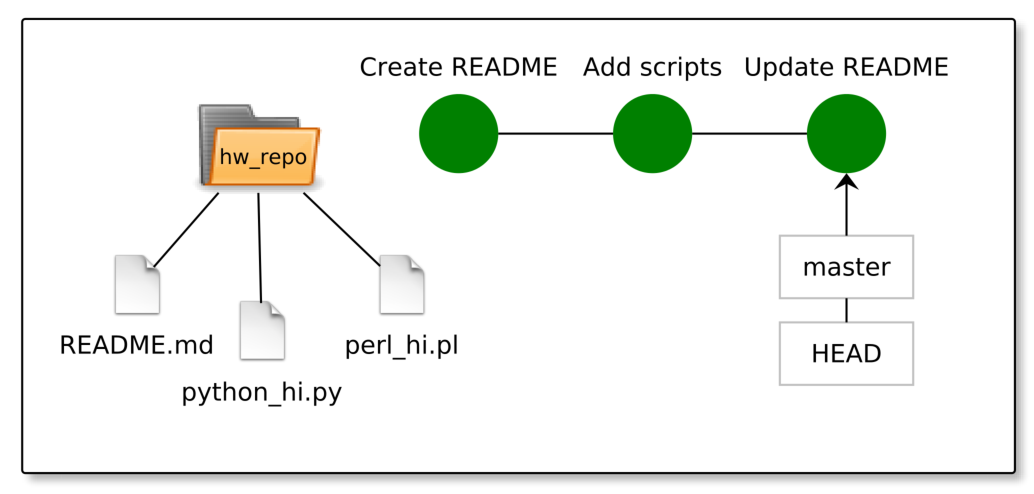
\includegraphics[width=0.8\textwidth]{../visualizations/chapter2/c26_repo_third_commit.pdf}
	\caption{State of repository before branching}
	\label{fig:state_before_branching}
\end{figure}

We create the new branch by initiating a new \verb$head$ at the current commit. To initiate the head, we use the command \verb$git branch <branch name>$:

\begin{codebox}
\begin{lstlisting}
$ git log --oneline
6ab7792 Update README
7100d36 Add scripts
b58c6c3 Create README
$ git branch py_upgrade
\end{lstlisting}
\end{codebox}

We initiated a new branch named \verb$py_upgrade$. This resulted in the repository creating a new head. At this point, our repository looks like figure \ref{fig:branch_initiated}.

\begin{figure}[h!]
	\centering
	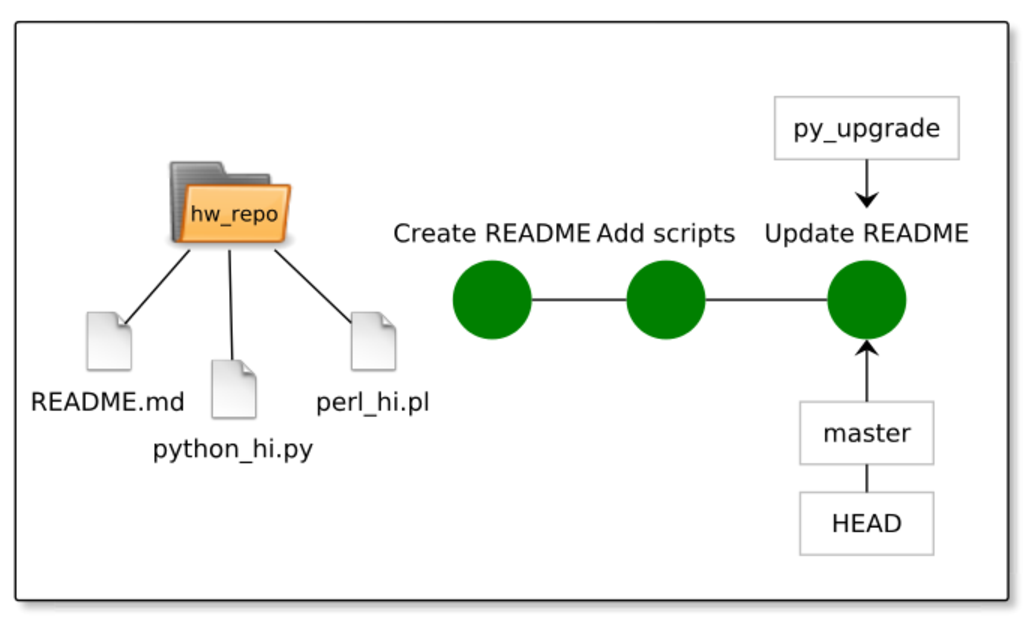
\includegraphics[width=0.8\textwidth]{../visualizations/chapter4/42_branch_initiated.pdf}
	\caption{State of with new branch initiated}
	\label{fig:branch_initiated}
\end{figure}

We have only created a new head at this point - there are no commits added to the branch and our \verb$HEAD$ still refers to the \verb$master$ branch. If we want to start working with the new branch, we need to switch \verb$HEAD$ to \verb$py_upgrade$.

We can see all available branches using the \verb$git branch$ without any
input. The asterisk shows where the \verb$HEAD$ is currently pointing.
Let's switch to our new branch using the \verb$git checkout$ command.

\begin{codebox}
\begin{lstlisting}
$ git branch
* master
  py_upgrade
$ git checkout py_upgrade
Switched to branch 'py_upgrade'
$ git branch 
  master
* py_upgrade
\end{lstlisting}
\end{codebox}

Let's make a new feature for the Python-script. In this case, the script was opened in the \verb$nano$ text editor. The \verb$cat$ command is used to show the file after the edits were completed.

\begin{codebox}
\begin{lstlisting}
$ nano python_hi.py
$ cat python_hi.py
#!/usr/bin/python3
import random
print("Hello world")
if random.random() > 0.5:
    print("Again: Hello world!!")
\end{lstlisting}
\end{codebox}

The Python script now randomly adds an extra "Hello world!" half of the times it is run. Next, we stage and commit the changes.

\begin{codebox}
\begin{lstlisting}
$ git add python_hi.py
$ git commit -m "Upgrade py"
[py_upgrade 159c0db] Upgrade py
 1 file changed, 3 insertions(+)
$ git log --oneline
159c0db Upgrade py
6ab7792 Update README
7100d36 Add scripts
b58c6c3 Create README
\end{lstlisting}
\end{codebox}

We added a new commit containing our new feature. Figure \ref{fig:branch_commit} shows the repository at this point.

\begin{figure}[h!]
	\centering
	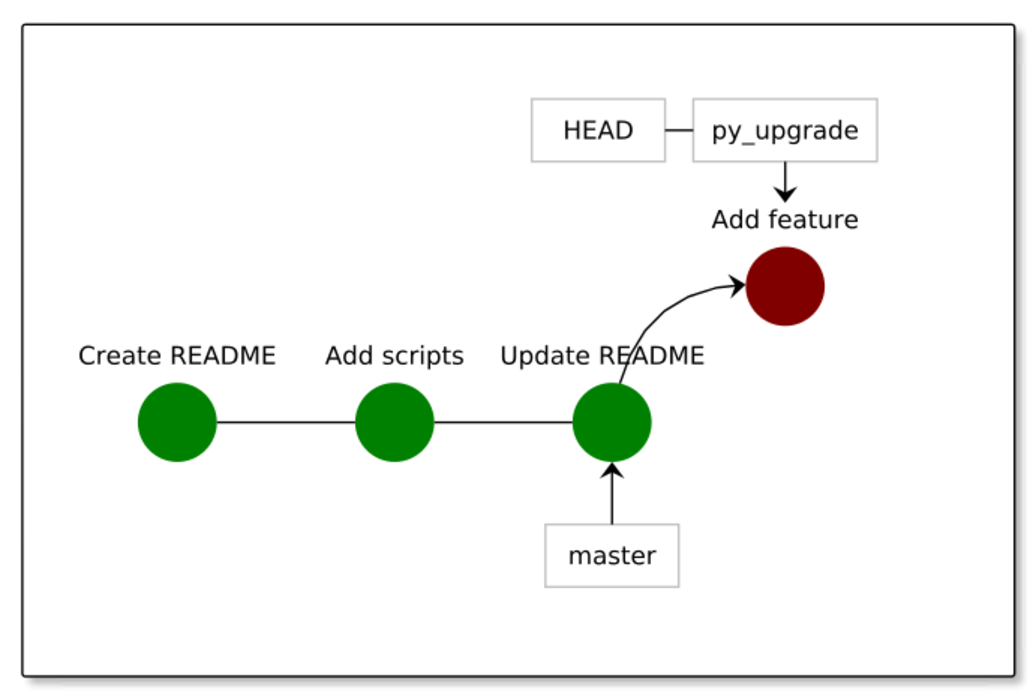
\includegraphics[width=0.8\textwidth]{../visualizations/chapter4/43_branch_with_commit.pdf}
	\caption{Branch with added commit}
	\label{fig:branch_commit}
\end{figure}

\begin{figure}[h!]
\begin{redbox}
Note that the current file tree represents the state of the repository where the HEAD is pointing. If we go back to the \verb$master$ head, we will return to the state of the files before we started developing our new feature.
\end{redbox}
\end{figure}

\begin{figure}[h!]
\begin{bluebox}
Command: \verb$git branch [<head-name>] [<starting-point>]$ \\

Creates a new head with the given name and point that to the given commit object.
If no starting-point argument is supplied, the branch will created from the current commit (\verb$git branch branch_name$).

If used without supplied argument, it will list available branches (\verb$git branch$).
\end{bluebox}
\label{command:branch}
\caption{git branch - Create a new branch in your repository}
\end{figure}

\subsection{Merging branches}

It is time to merge our changes back into the master branch.
To do this, we use the \verb$git merge$ command. \verb$git merge$ incorporates the changes made by the other branch into the current branch.
It will create a new commit, and both the heads will end up pointing to the same commit.

\begin{figure}[h!]
\begin{bluebox}
Command: \verb$git merge <branch_to_merge>$ \\

Merges the given branch into the currently active branch.
\end{bluebox}
\label{command:merge}
\caption{git merge - Merge a branch into the current branch}
\end{figure}

Let's merge our changes back into the \verb$master$. There are no conflicts here
which will make the re-merge smooth and pain-free.

\begin{codebox}
\begin{lstlisting}
$ git checkout master
Switched to branch 'master'
$ git merge py_upgrade
Updating 6ab7792..159c0db
Fast-forward
 python_hi.py | 3 +++
 1 file changed, 3 insertions(+)
\end{lstlisting}
\end{codebox}

No problems here - A new commit was created implementing the changes to the \verb$new_feature$ branch into the \verb$master$. Figure \ref{fig:smooth_merge} shows the repository at this stage.

\begin{figure}[h!]
	\centering
	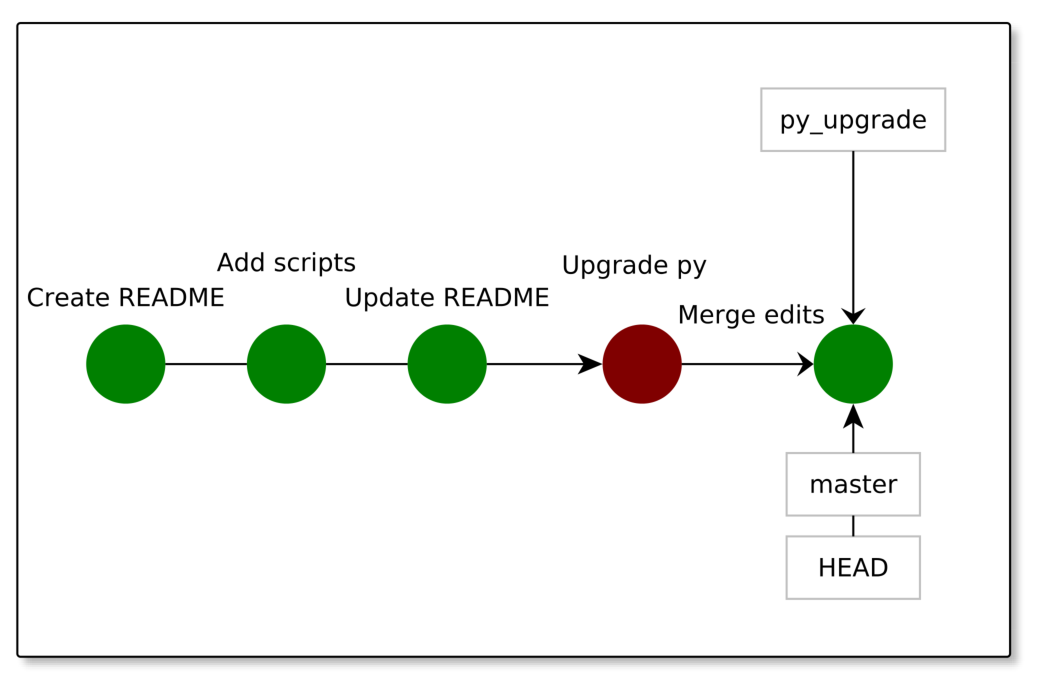
\includegraphics[width=0.8\textwidth]{../visualizations/chapter4/44_smoothly_merged_branch.pdf}
	\caption{Smoothly merged repository}
	\label{fig:smooth_merge}
\end{figure}

\subsection{Dealing with merge conflicts}

The previous merge went smoothly as we didn't have any conflicting changes (changes made to the same part of the same file) made between the branches. Now, let's see what happens if we try to merge our branches back together after doing some conflicting changes. We now back up to the state of the repository shown in figure \ref{fig:state_before_branching}.

\begin{figure}[h!]
\begin{redbox}
For ease-of-presentation, the repository has been reverted to its state before performing the merge in the example below. This means that you aren't able to exactly trace the state used in the example. It is recommended that you add a new commit to your branch, and then create a parallel edit on your master in order to try out solving a merge conflict.
\end{redbox}
\end{figure}

Let's do another set of changes to induce a merge conflict. Remove the previous branch, and create a new one.

\begin{codebox}
\begin{lstlisting}
$ git branch -d py_upgrade
Deleted branch py_upgrade (was 508edb8).
$ git branch py_upgrade2
\end{lstlisting}
\end{codebox}

Let's do some changes to the master branch.

\begin{codebox}
\begin{lstlisting}
$ nano python_hi.py
$ cat python_hi.py
#!/usr/bin/python3
import random
print("Hello world")
print("Hello from master!")
if random.random() > 0.5:
    print("Again: Hello world!!")
$ git add python_hi.py
$ git commit -m "Master hi"
[py_upgrade2 032cac1] Master hi
 1 file changed, 1 insertion(+)
\end{lstlisting}
\end{codebox}

Now, switch to the branch and do parallel edits.

\begin{codebox}
\begin{lstlisting}
$ git checkout py_upgrade2
Switched to branch 'py_upgrade2'
$ git branch
  master
* py_upgrade2
$ nano python_hi.py
$ cat python_hi.py
#!/usr/bin/python3
import random
print("Clashing edits!")
if random.random() > 0.5:
    print("Again: Hello world!!")
$ git add python_hi.py
$ git commit -m "Create clash"
[master 4241ef3] Create clash
 1 file changed, 1 insertion(+), 1 deletion(-)
\end{lstlisting}
\end{codebox}

Switch back to the master branch.

\begin{codebox}
\begin{lstlisting}
$ git checkout master
Switched to branch 'master'
$ git branch
* master
  py_upgrade2
\end{lstlisting}
\end{codebox}

Now, we have parallel changes on the \verb$py_upgrade2$-branch and on the \verb$master$-branch. The state of our repository is shown in figure \ref{fig:before_conflict_merge}.

\begin{figure}[h!]
	\centering
	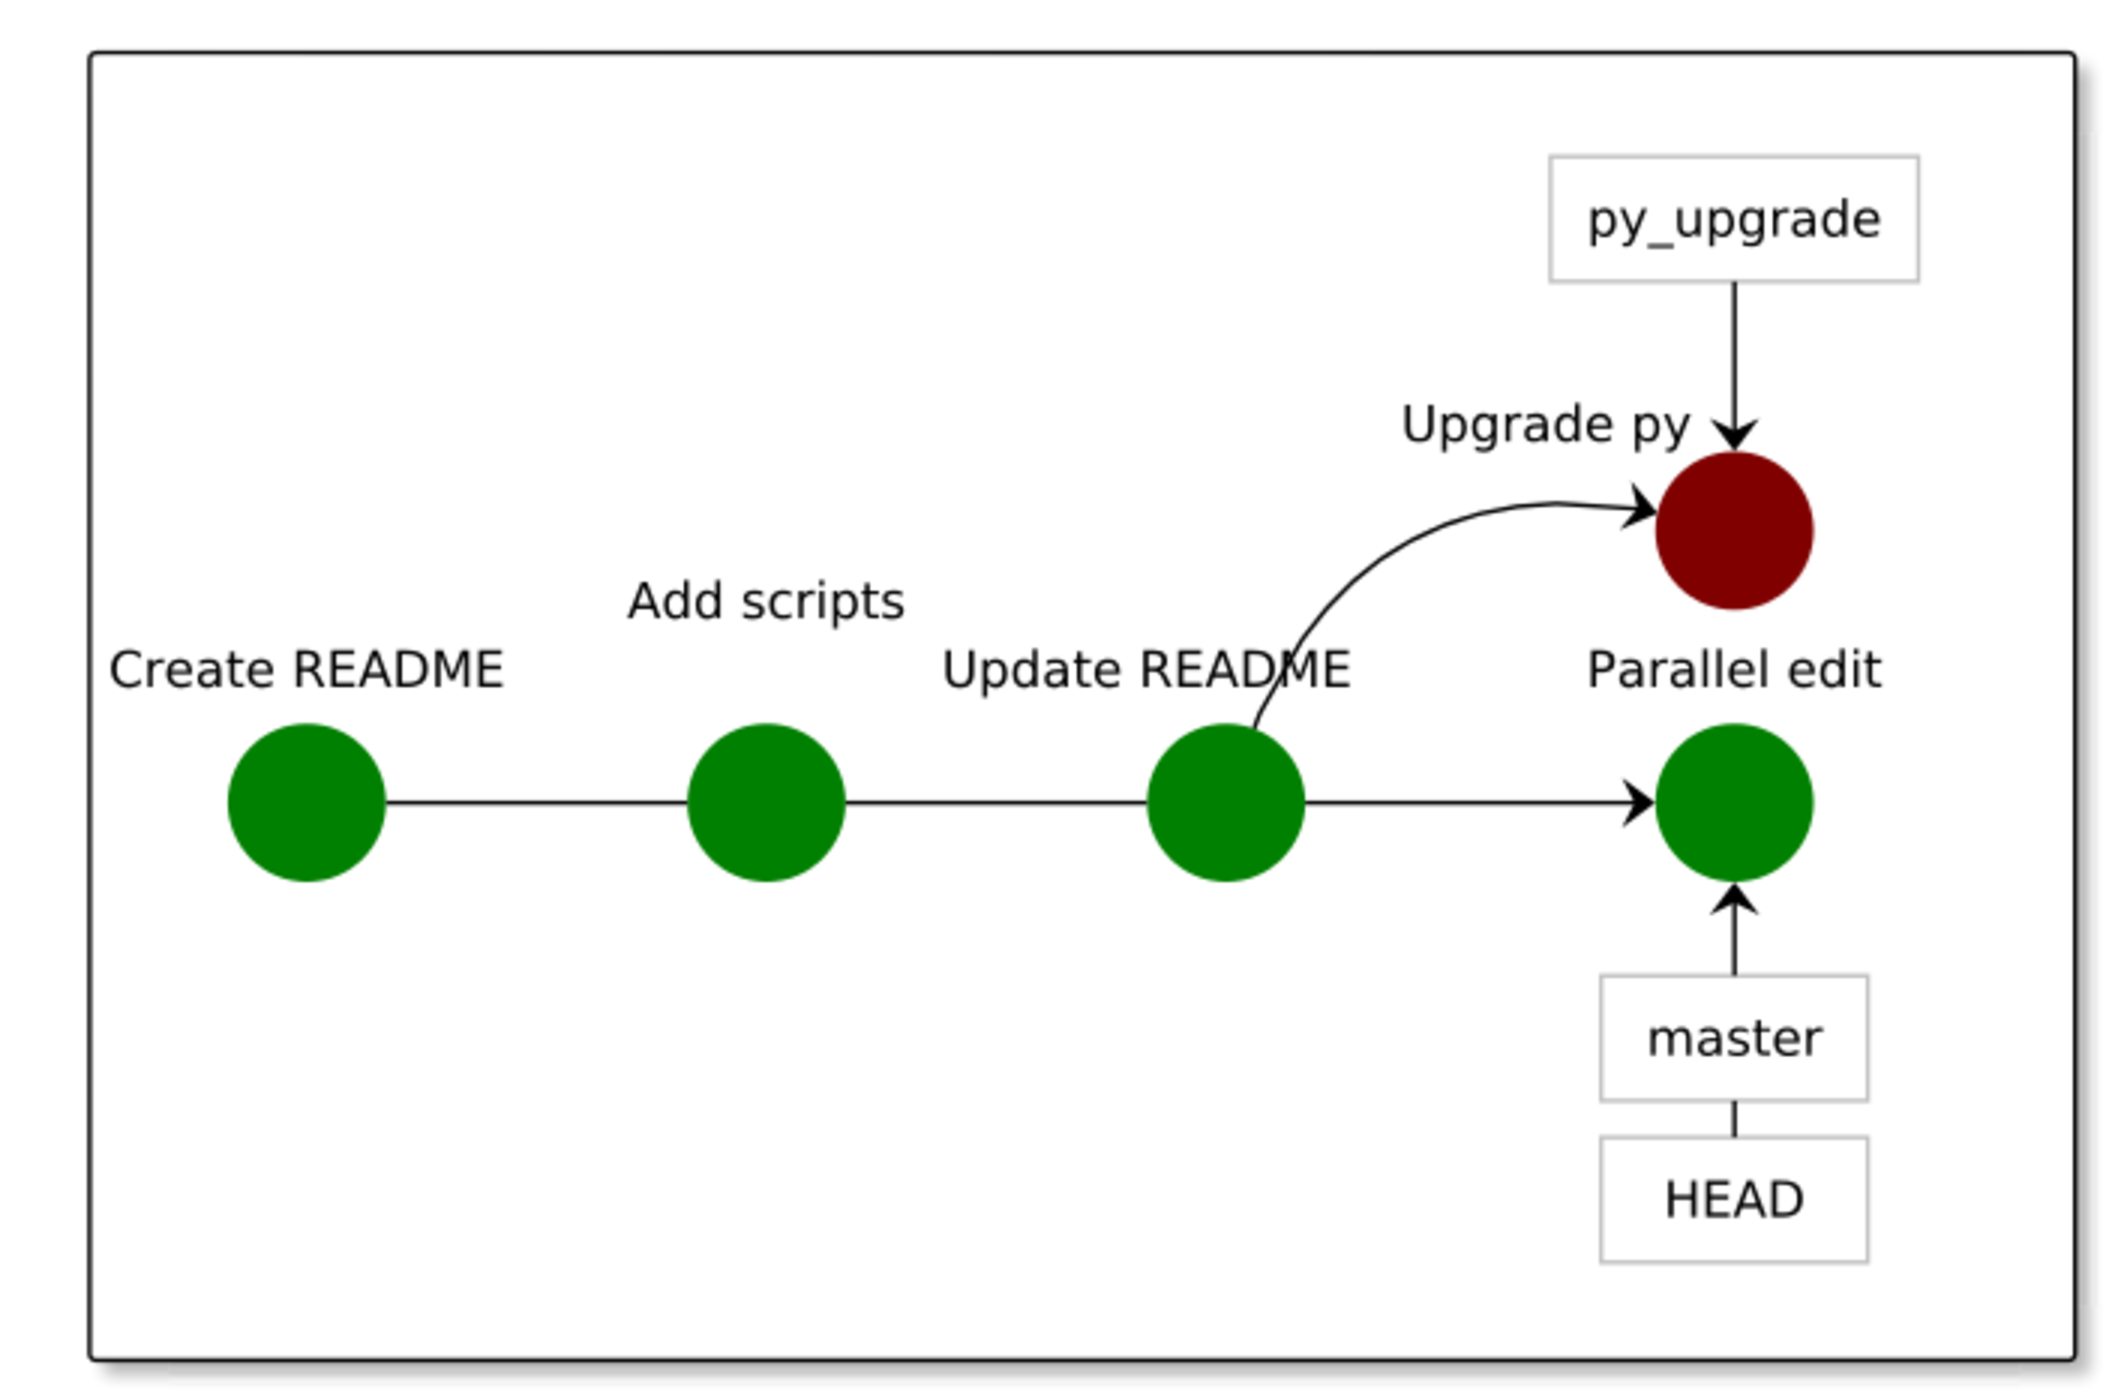
\includegraphics[width=0.8\textwidth]{../visualizations/chapter4/45_parallel_edits_on_master_branch}
	\caption{Parallel edits on master and branch}
	\label{fig:before_conflict_merge}
\end{figure}

If the changes are made in different files, or even in different parts of the same
file, no merge conflicts will occur. The default text editor will be opened,
and you will be able to enter a commit message for the merge commit.

If you on the other hand have merge conflicts by editing the same file in the same place (as we do here), you need to manually pick the edits you want to use.

\begin{codebox}
\begin{lstlisting}
$ git merge py_upgrade2
Auto-merging python_hi2.py
CONFLICT (content): Merge conflict in python_hi2.py
Automatic merge failed; fix conflicts and then commit the 
result.
\end{lstlisting}
\end{codebox}

You will have to
resolve this manually, either by editing the file directly or using a merge-tool.
Here, we will edit the file directly. It is also possible to use dedicated merge-tools like \textit{meld} (\url{http://meldmerge.org/}), but for these examples editing the text files directly is definitely enough. 

\begin{codebox}
\begin{lstlisting}
$ git status
On branch master
You have unmerged paths.
  (fix conflicts and run "git commit")
  (use "git merge --abort" to abort the merge)

Unmerged paths:
  (use "git add <file>..." to mark resolution)

        both modified:      python_hi.py
        
no changes added to commit (use "git add" and/or "git commit 
-a")
$ cat python_hi.py
#!/usr/bin/python3
import random
<<<<<<< HEAD
print("Clashing edits!")
=======
print("Hello world")
print("Hello from master!")
>>>>>>> py_upgrade2
if random.random() > 0.5:
    print("Again: Hello world!!")
\end{lstlisting}
\end{codebox}

The lines between \verb$<<<<<< HEAD$ and \verb$=======$ are present in the current HEAD (in this case - the master branch). The lines between \verb$=======$ and \verb$>>>>>>> py_upgrade$ are present in the python\_hi\_upgrade-branch.

In this case, we would like to retain the changes made to the \verb$py_upgrade$ branch. To do this we simply remove the dividers inserted by Git (\verb$<<<$, \verb$===$ and \verb$>>>$), alongside with the lines that we don't want to keep.

\begin{codebox}
\begin{lstlisting}
$ nano python_hi.py  # Remove merge-lines and "Clashing edits"
$ cat python_hi.py
#!/usr/bin/python3
import random
print("Hello world")
print("Hello from master!")
if random.random() > 0.5:
    print("Again: Hello world!!")
$ git add python_hi.py
$ git commit -m "Merging edits"
[master 791e895] Merge edits
\end{lstlisting}
\end{codebox}

Now, we have all the history in place, and our changes has been merged into the master branch.
At this point, our repository looks like the following:

\begin{figure}[h!]
	\centering
	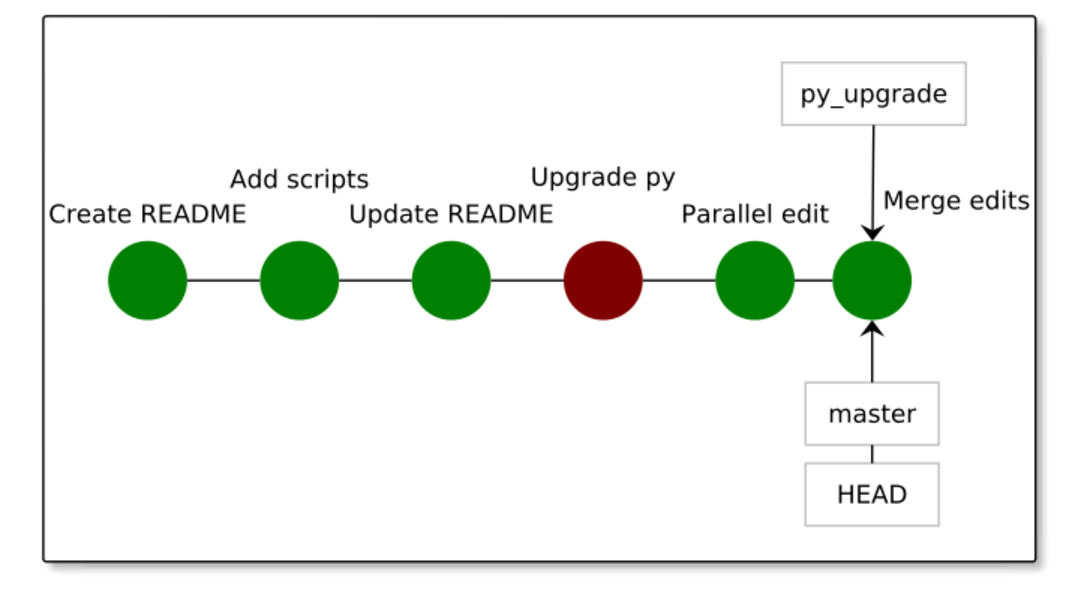
\includegraphics[width=0.8\textwidth]{../visualizations/chapter4/46_successful_merge_post_conflict.pdf}
	\caption{Successful merge after merge conflict}
	\label{fig:after_merged_conflict}
\end{figure}

Note that the \verb$py_upgrade$ branch is still there, even if it has been merged back into the master.
If we don't want to use it any more we could simply remove it from the repository.

\begin{codebox}
\begin{lstlisting}
$ git branch
* master
  py_upgrade
$ git branch -d py_upgrade
Deleted branch py_upgrade (was 159c0db).
$ git branch
* master
\end{lstlisting}
\end{codebox}

\newpage
\section{Exercises}

The exercises presented here will work fine for any repository. You could either continue using the repository you built in the previous chapters, or create a new one.

The concepts of this chapter are important, especially understanding merge-conflicts which occurs both when working with branches and remote repositories. With that said, if you are short on time, make sure that you make it through Chapter 5. Then you could return here at a later point.

\subsection{Using branching (*)}

Here, we will go through the steps for branching that were explained in the previous text. If you get stuck, or aren't sure on the meaning of the steps, take a look into the previous text.

\begin{enumerate}
	\item Run the \verb$git branch$ command and check what branches are present in your repository before initiating new branches.
	\item Create a new branch for a new feature you want to implement. Check the output of \verb$git branch$.
	\item Switch to your new branch using the command \verb$git checkout$. Check the output of \verb$git branch$. Remember, Git will protest if you have any uncommitted changes.
	\item Implement a new feature using one or more commits, preferably including changes to at least one of your existing files.
	\item Return to the master by running \verb$git checkout$.
	\item Now, add some commits to your master. Make sure to include some edits to the same files which you worked with on your branch, with at least one edit directly clashing with the edits made on the branch.
	\item Let's merge the feature branch back into the master using \verb$git merge$. Before merging, stop for a moment, and visualize the current state of the repository and the file tree. How will they look before and after performing the merge?
	\item Perform the merge. You will likely need to make a merge commit. You can check the current status using \verb$git status$. Do you have any files for which the merge failed? (Written as "both modified" in the \verb$git status$ output). Resolve the conflicts by inspecting the files and removing the lines that you don't want to keep.	
\end{enumerate}

Merge conflicts can be a particularly confusing part when getting starting with Git. When you encounter a merge conflict, make sure that you understand what is going on and what you want to accomplish. You can always refer to this material if you are unsure on what is going on.

\subsection{Further branching (*)}

\begin{itemize}
	\item The asterisk in the \verb$git branch$ output shows you the currently active branch. What output do you get if you check out a commit not related to a branch? What does it mean?
	\item Visualize the steps of the previous exercise. Make sure that you have a good understanding of what happens with the file tree, repository and heads when running each of the commands.
\end{itemize}

% Create another repository
% Add some commits, make sure you follow what you are doing
% Add two branches, and do some commits - Can you visualize your repo?
% Merge the branches back into the master
% Create another branch, make one commit, and deliberately insert merge conflicts
% Try merging back again
% Solve the conflict
% Clean up your repository by removing unwanted branches

\newpage
\section{Recap}

\subsection{Concepts}

\begin{itemize}
	\item Can you name one or more potential purposes of branches in Git?
	\item What is a merge conflict, and when does it occur?
\end{itemize}

\subsection{Commands}

\begin{itemize}
	\item \verb$git branch [<branch_name>] [<target_commit>]$
	\item \verb$git branch -d <branch_name>$
	\item \verb$git merge <branch_name>$
	\item \verb$git checkout <branch_name>$
\end{itemize}

\end{document}
